\normaltrue \difficilefalse \tdifficilefalse
\correctiontrue

%\UPSTIidClasse{11} % 11 sup, 12 spé
%\newcommand{\UPSTIidClasse}{11}

\exer{Diagramme de Bode$\star$ \label{C2:02:510_02}}
\setcounter{question}{0}\UPSTIcompetence[2]{C2-02}
\index{Compétence C2-02}
\index{Diagramme de Bode}
\ifcorrection
\else
\marginnote{\textbf{Pas de corrigé pour cet exercice.}}
\fi




\question{Tracer le diagramme de Bode de la fonction de transfert suivante : $F_2(p)=\dfrac{10}{\left(1+10p\right)\left(10+p\right)}$.}
\ifprof
\textbf{Tracer asymptotique}

$F_2(p)=\dfrac{1}{\left(1+10p\right)\left(1+\dfrac{p}{10}\right)}$

\begin{center}
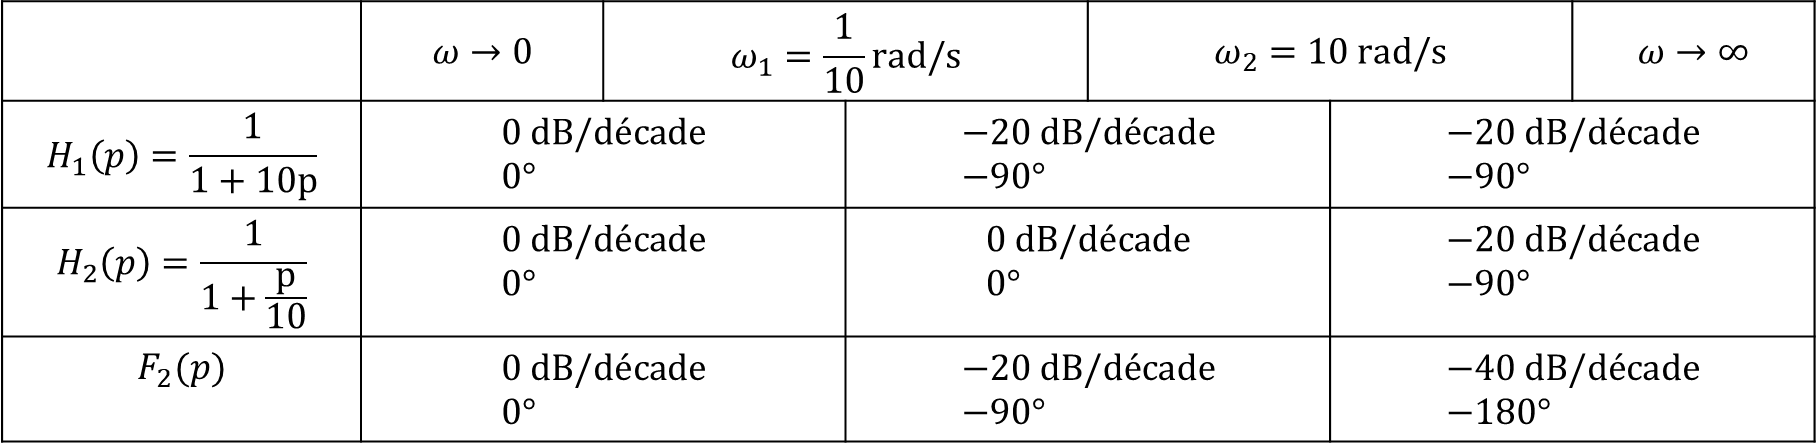
\includegraphics[width=.9\linewidth]{tab_02}
\end{center}


\textbf{Positionnement du diagramme de gain}
Lorsque que $\omega$ tend vers 0, le gain tend vers $20 \log 1 = \SI{0}{dB}$.


\begin{center}
 \begin{tikzpicture}[xscale=1.5]
\tikzset{
semilog lines/.style={thin, bleuxp}, 
semilog lines 2/.style={semilog lines,bleuxpc},
semilog half lines/.style={semilog lines 2,dotted },
semilog label x/.style={semilog lines,below,font=\tiny,black},
semilog label y/.style={semilog lines,right,font=\tiny,black}
}
\begin{scope}[yscale=1/40]
\semilog{-3}{3}{-140}{20}
\UnitedB
\OrdBode{20}
\BodeAmp[orangexp,thin,samples=100]{-3:3}{\POAmpAsymp{1}{10} + \POAmpAsymp{1}{10}}
\BodeAmp[orangexp,ultra thick]{-3:3}{\POAmp{1}{10} + \POAmp{1}{0.1}}

%\draw (-2.2,27) node {\footnotesize 23,5 dB, 0 dB/d\'ecade};
%\draw (.3,15) node {\footnotesize $-$20 dB/d\'ecade};
%\draw [dashed,ultra thick,bleuxp] (-1,-1) -- (-1,23.5);
%\draw (-1,-1)  node {\Huge $\cdot$} node [above right]{\footnotesize 0,1};
\end{scope}

\begin{scope}[yshift=-5cm,yscale=1/90]
\UniteDegre
\OrdBode{45}
\semilog{-3}{3}{-180}{90}
\BodeArg[orangexp,samples=101,thin]{-3:3}{\POArgAsymp{1}{10} + \POArgAsymp{1}{0.1}}
\BodeArg[orangexp,ultra thick]{-3:3}{\POArg{1}{10} + \POArg{1}{0.1}}
\end{scope}
\end{tikzpicture}
\end{center}
%
%\begin{center}
%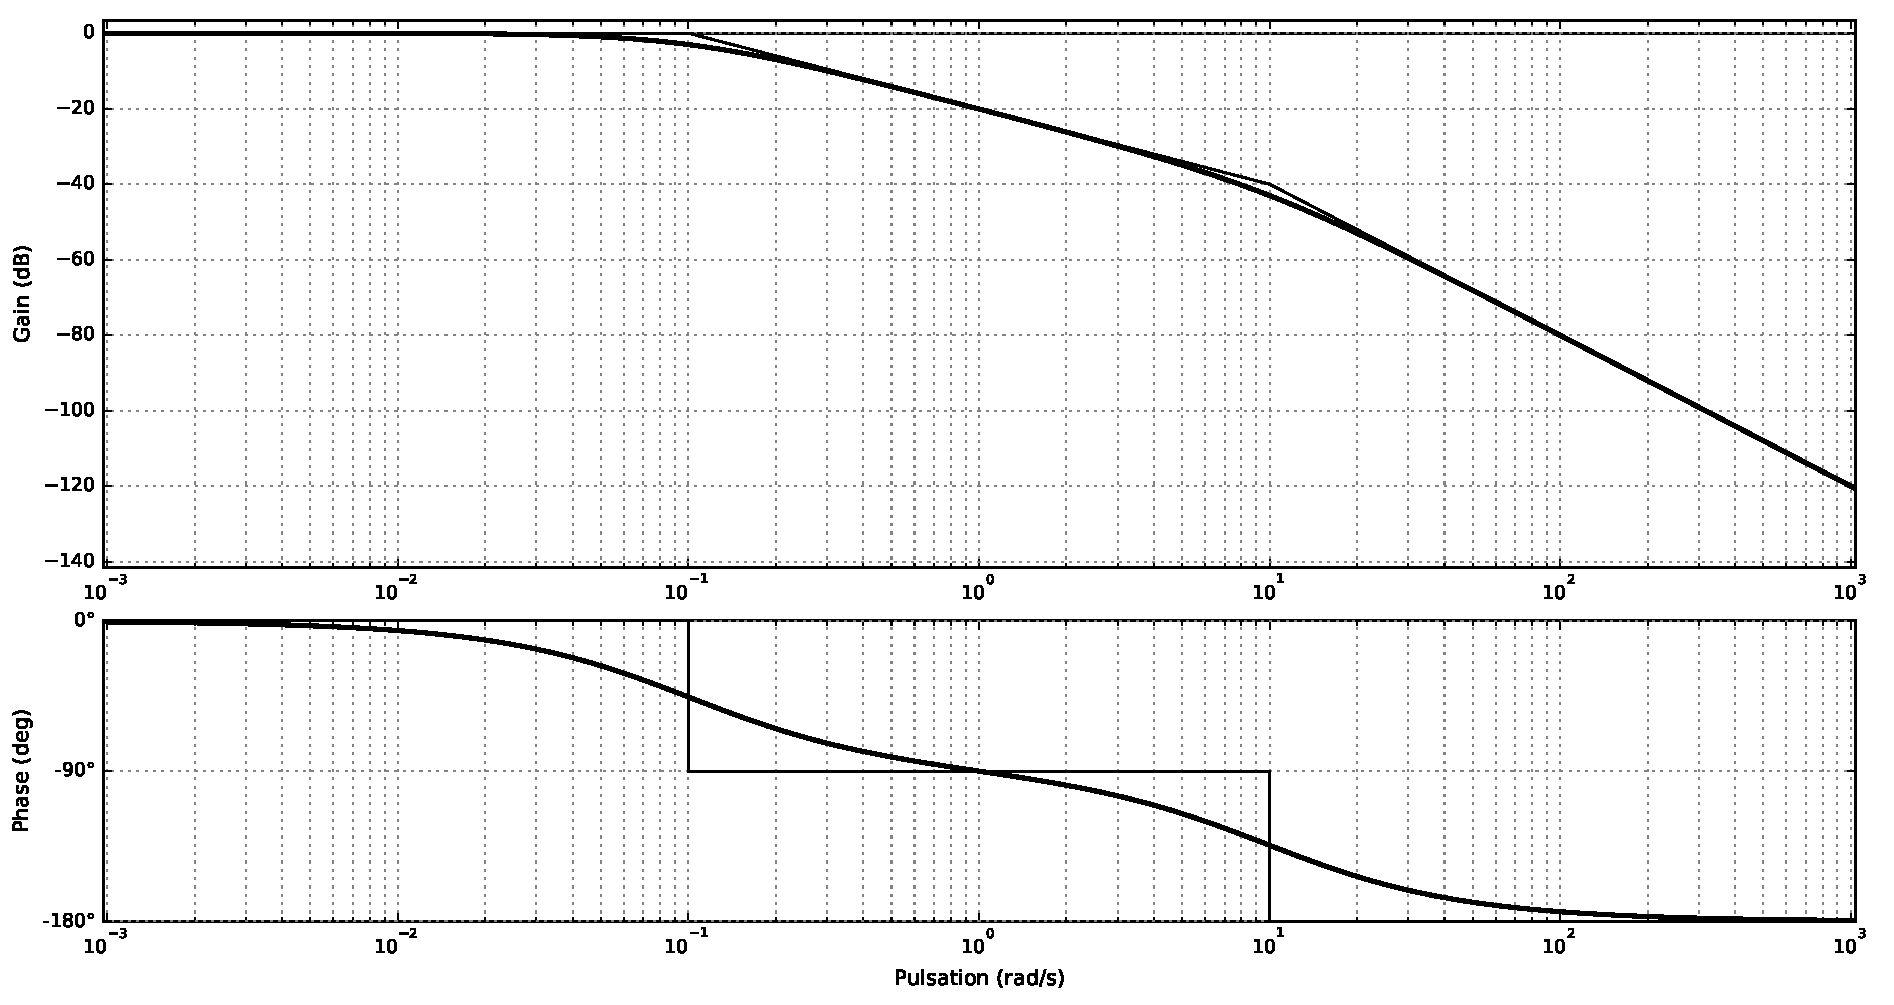
\includegraphics[width=.9\linewidth]{bode_02}
%\end{center}

\else 
%\begin{center}
%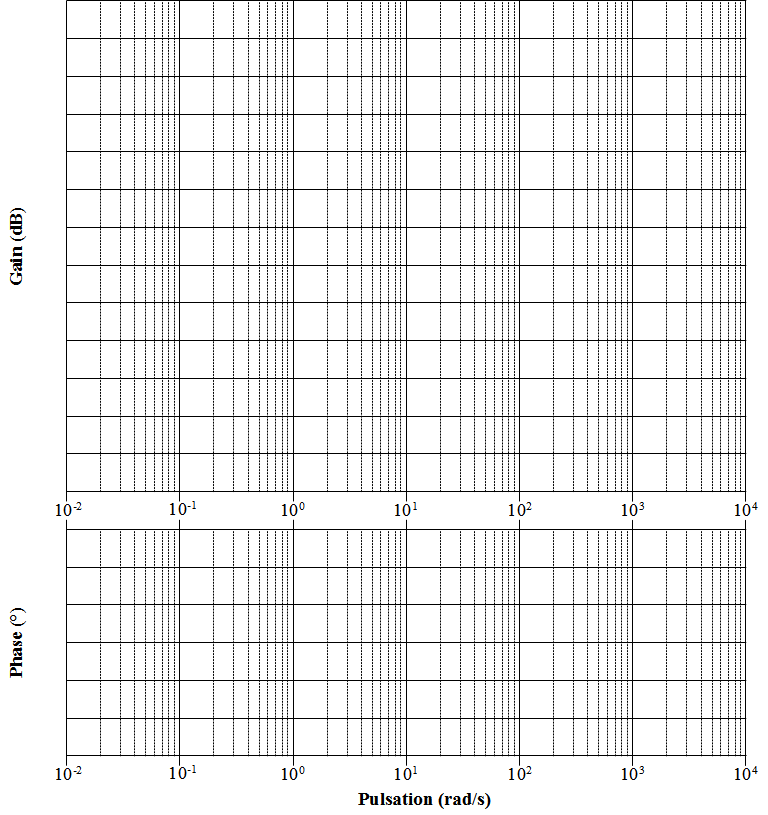
\includegraphics[width=.9\linewidth]{510_01}
%\end{center}
\begin{center}
 \begin{tikzpicture}[xscale=1.5]
\tikzset{
semilog lines/.style={thin, bleuxp}, 
semilog lines 2/.style={semilog lines,bleuxpc},
semilog half lines/.style={semilog lines 2,dotted },
semilog label x/.style={semilog lines,below,font=\tiny,black},
semilog label y/.style={semilog lines,right,font=\tiny,black}
}
\begin{scope}[yscale=1/40]
\semilog{-3}{3}{-140}{20}
\UnitedB
\OrdBode{20}

\end{scope}

\begin{scope}[yshift=-5cm,yscale=1/90]
\UniteDegre
\OrdBode{45}
\semilog{-3}{3}{-180}{90}
\end{scope}
\end{tikzpicture}
\end{center}
\fi


\question{Le système est sollicité par une entrée sinusoïdale de période \SI{6}{s} et d'amplitude 10. Quel est le signal de sortie ?}
\ifprof
Pour une période de \SI{60}{s}, la pulsation est de $\dfrac{2\pi}{T}$ soit $\omega = \SI{0,1}{rad.s^{-1}}$.
Pour cette pulsation le gain est de \SI{-5}{dB} et le déphasage de $-\dfrac{\pi}{4}$.

On a donc $20\log(S/E) = -5$ soit $S=E\times 10^{-5/20}=10\times 0,56 = 5,6$. Le signal d'entrée est donc $e(t) = 10 \sin (0,1 t)$ et le signal de sortie  
$s(t) = 5,6 \sin\left(0,1 t - \dfrac{\pi}{4}\right)$.
\else
\fi



\ifprof
\else
\begin{flushright}
\footnotesize{Corrigé  voir \ref{C2:02:510_02}.}
\end{flushright}%
\fi